\begin{frame}{Цель работы}
\phantomsection\label{ux446ux435ux43bux44c-ux440ux430ux431ux43eux442ux44b}
Освоить набор математических формул в LaTeX, изучить математические
режимы и работу с пакетами для математической верстки.
\end{frame}

\begin{frame}{Задание}
\phantomsection\label{ux437ux430ux434ux430ux43dux438ux435}
\begin{enumerate}
\tightlist
\item
  Изучить математические режимы LaTeX
\item
  Освоить верхние и нижние индексы
\item
  Изучить греческие буквы и функции
\item
  Научиться работать с уравнениями и матрицами
\item
  Выполнить практические упражнения
\end{enumerate}
\end{frame}

\begin{frame}[fragile]{Основные математические режимы}
\phantomsection\label{ux43eux441ux43dux43eux432ux43dux44bux435-ux43cux430ux442ux435ux43cux430ux442ux438ux447ux435ux441ux43aux438ux435-ux440ux435ux436ux438ux43cux44b}
\textbf{Два основных режима:} - Инлайн-режим:
\texttt{\$y\ =\ mx\ +\ c\$} - Дисплей-режим:
\texttt{\textbackslash{}{[}\ y\ =\ mx\ +\ c\ \textbackslash{}{]}}

\begin{figure}
\centering
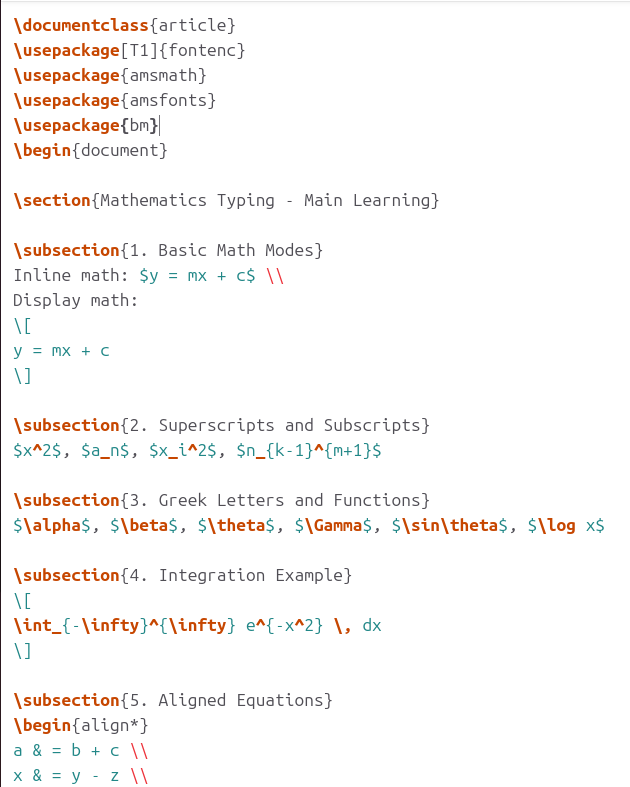
\includegraphics[width=0.5\textwidth,height=\textheight]{image_02.jpg}
\caption{Пример математического кода}
\end{figure}
\end{frame}

\begin{frame}[fragile]{Создание основного документа}
\phantomsection\label{ux441ux43eux437ux434ux430ux43dux438ux435-ux43eux441ux43dux43eux432ux43dux43eux433ux43e-ux434ux43eux43aux443ux43cux435ux43dux442ux430}
Создал файл \texttt{math-practice.tex} с математическими конструкциями:

\begin{itemize}
\tightlist
\item
  Верхние и нижние индексы
\item
  Греческие буквы
\item
  Интегралы и уравнения
\item
  Матрицы и шрифты
\end{itemize}

\begin{figure}
\centering
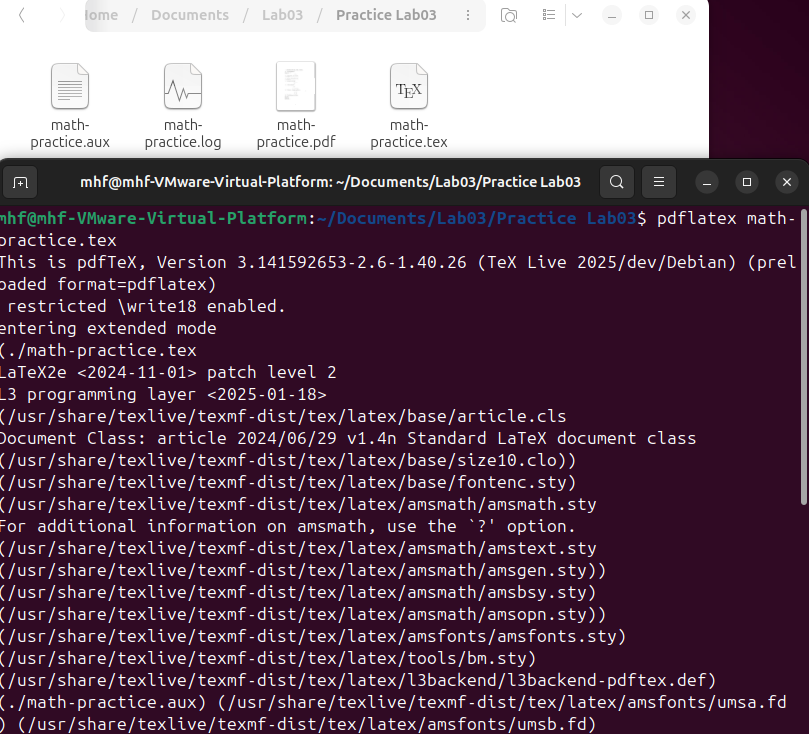
\includegraphics[width=0.5\textwidth,height=\textheight]{image_01.jpg}
\caption{Процесс компиляции}
\end{figure}
\end{frame}

\begin{frame}[fragile]{Компиляция документа}
\phantomsection\label{ux43aux43eux43cux43fux438ux43bux44fux446ux438ux44f-ux434ux43eux43aux443ux43cux435ux43dux442ux430}
Процесс компиляции основного документа:

\begin{Shaded}
\begin{Highlighting}[]
\ExtensionTok{pdflatex}\NormalTok{ math{-}practice.tex}
\end{Highlighting}
\end{Shaded}

Результат - успешная компиляция без ошибок

\begin{figure}
\centering
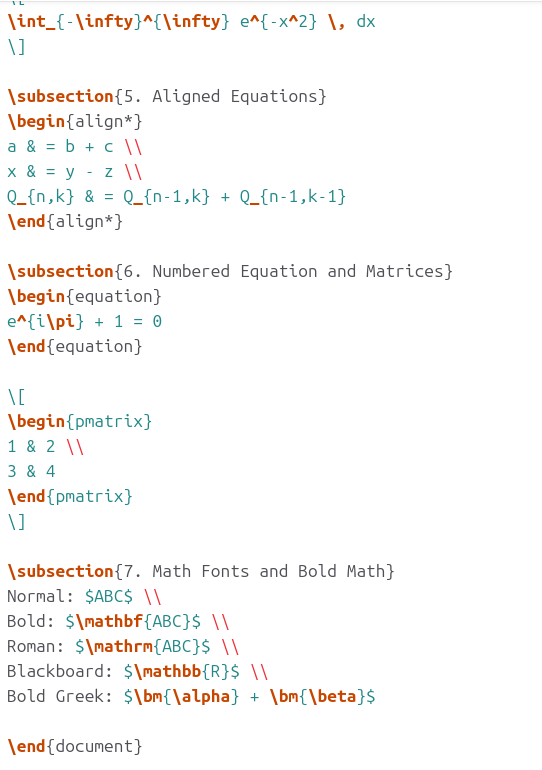
\includegraphics[width=0.7\textwidth,height=\textheight]{image_03.jpg}
\caption{Отладка математических формул}
\end{figure}
\end{frame}

\begin{frame}{Практические упражнения}
\phantomsection\label{ux43fux440ux430ux43aux442ux438ux447ux435ux441ux43aux438ux435-ux443ux43fux440ux430ux436ux43dux435ux43dux438ux44f}
Создал файл exercises.tex с 4 упражнениями:

Сравнение инлайн и дисплей режимов

Практика с греческими буквами

Исследование шрифтов

Опции документа

\begin{figure}
\centering
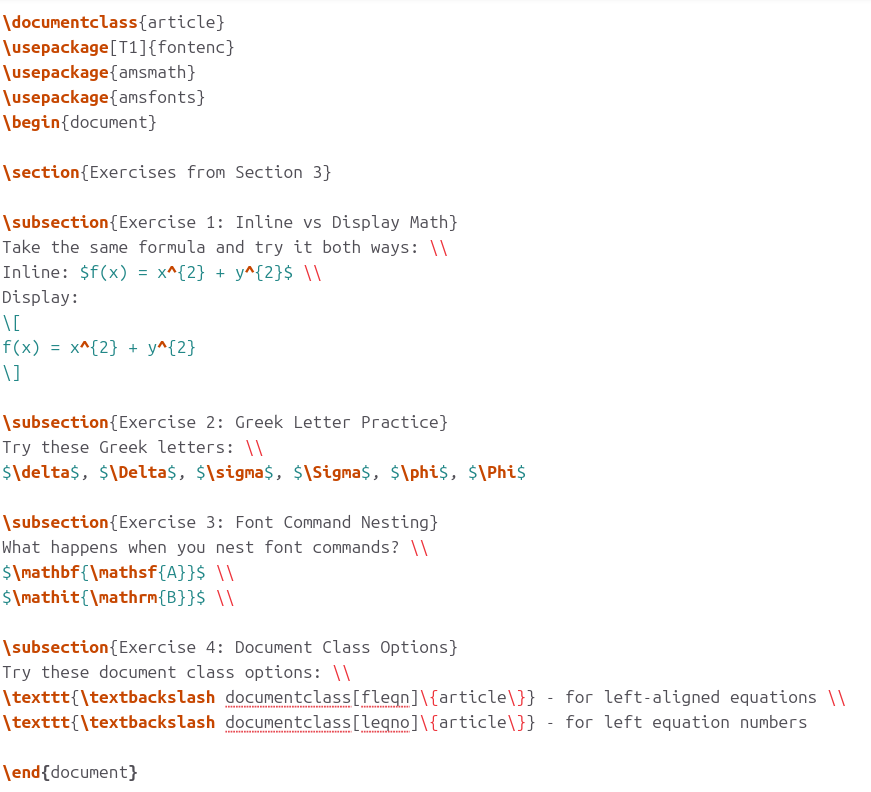
\includegraphics[width=0.7\textwidth,height=\textheight]{image_06.jpg}
\caption{Исходный код документа с упражнениями}
\end{figure}
\end{frame}

\begin{frame}[fragile]{Компиляция упражнений}
\phantomsection\label{ux43aux43eux43cux43fux438ux43bux44fux446ux438ux44f-ux443ux43fux440ux430ux436ux43dux435ux43dux438ux439}
Выполнил компиляцию упражнений:

\begin{Shaded}
\begin{Highlighting}[]
\ExtensionTok{pdflatex}\NormalTok{ exercises.tex}
\end{Highlighting}
\end{Shaded}

\begin{figure}
\centering
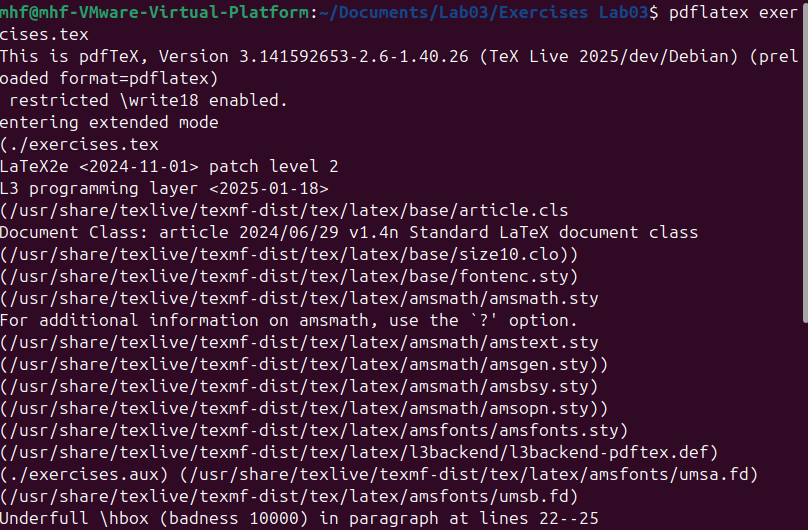
\includegraphics[width=0.7\textwidth,height=\textheight]{image_05.jpg}
\caption{Процесс компиляции упражнений}
\end{figure}
\end{frame}

\begin{frame}{Изученные математические элементы}
\phantomsection\label{ux438ux437ux443ux447ux435ux43dux43dux44bux435-ux43cux430ux442ux435ux43cux430ux442ux438ux447ux435ux441ux43aux438ux435-ux44dux43bux435ux43cux435ux43dux442ux44b}
Изученные математические элементы Основные элементы:

Верхние/нижние индексы: \(x^2\), \(a_n\)

Греческие буквы: \(\alpha\), \(\beta\), \(\Gamma\)

Функции: \(\sin\theta\), \(\log x\)

Интегралы: \(\int e^{-x^2} dx\)

Матрицы: pmatrix, bmatrix

Шрифты: \(\mathbf{B}\), \(\mathbb{R}\), \(\mathrm{C}\)

\begin{figure}
\centering
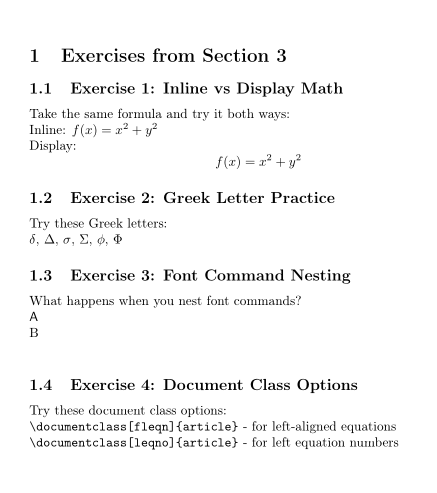
\includegraphics[width=0.7\textwidth,height=\textheight]{image_07.jpg}
\caption{Альтернативная версия кода упражнений}
\end{figure}
\end{frame}

\begin{frame}{Специальные математические команды}
\phantomsection\label{ux441ux43fux435ux446ux438ux430ux43bux44cux43dux44bux435-ux43cux430ux442ux435ux43cux430ux442ux438ux447ux435ux441ux43aux438ux435-ux43aux43eux43cux430ux43dux434ux44b}
Изученные команды:

\(\frac{a}{b}\) - дроби

\(\sum\), \(\prod\) - суммы и произведения

\(\lim\), \(\int\) - пределы и интегралы

\textbackslash begin\{align*\} - выровненные уравнения

\textbackslash begin\{pmatrix\} - матрицы

\(\mathbf{A}\) - жирный шрифт
\end{frame}

\begin{frame}{Результаты работы}
\phantomsection\label{ux440ux435ux437ux443ux43bux44cux442ux430ux442ux44b-ux440ux430ux431ux43eux442ux44b}
Достигнутые результаты:

Успешная компиляция обоих документов

Освоены все математические режимы

Изучены греческие буквы и функции

Практика с матрицами и уравнениями

Выполнены все 4 упражнения

\begin{figure}
\centering
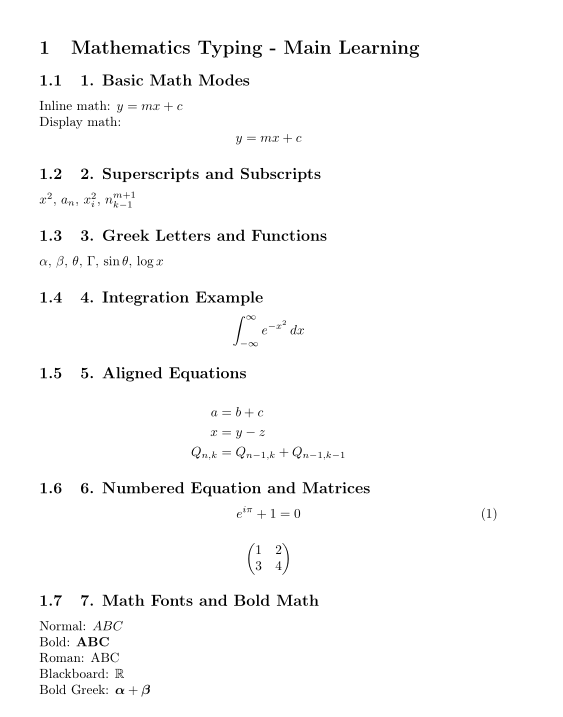
\includegraphics[width=0.7\textwidth,height=\textheight]{image_04.jpg}
\caption{Исходный код основного документа - попытка 2}
\end{figure}
\end{frame}

\begin{frame}{Выводы}
\phantomsection\label{ux432ux44bux432ux43eux434ux44b}
В ходе лабораторной работы №3:

Освоены математические режимы LaTeX

Изучены команды для сложных формул

Практически применены знания

Успешно созданы документы с математикой

Получены навыки работы с пакетом amsmath

Система LaTeX доказала свою эффективность для научных публикаций.
\end{frame}
